\chapter{Chocs de particules}

\section{D\'esint\'egration des particules}

Les lois de conservations ne d\'ependent absolument pas de l'esp\`ece d'interaction entre les particules et permettent ainsi d'arriver \`a des conclusions pourtant importantes pour les processus m\'ecaniques en jeu.

Pour commencer, choisissons la d\'esint\'egration spontan\'ee, i.e. non provoqu\'ee par des forces ext\'erieures, d'une particule en deux autres particules se d\'epla\c{c}ant apr\`es la d\'esint\'egration ind\'ependamment l'une de l'autre. Sa forme la plus simple est quand il est consid\'er\'e dans un syst\`eme de r\'ef\'erence o\`u la particule initiale est au repos. La conservation d' l'impulsions implique :
\bea
	\vec{p}_{1} + \vec{p}_{2} & = & \vec{0} \nonumber \\
	\vec{p}_{1} & = & -\vec{p}_{2}
\eea
ainsi les particules r\'esultantes de la d\'esint\'egration s'\'eloignent l'une de l'autre avec des impulsions \'egales, ,$\lVert \vec{p}_{1} \rVert = \lVert \vec{p}_{2} \rVert = p_{0}$ et dirig\'ees en sens inverse.

En utilisant la loi de conservation de l'\'energie et en particulier l'\'equation (\ref{EQ:8_4}) et parce que l'\'energie cin\'etique de la particule initiale est nulle, nous pouvons \'ecrire :
\be
	E_{int} = E_{1int} + \dfrac{p_{0}^{2}}{2m_{1}} + E_{2int} + \dfrac{p_{0}^{2}}{2m_{2}}
\ee
avec $E_{int}$ l'\'energie interne de la particule initiale, $E_{1int}$ et $E_{2int}$ l'\'energie interne des deux particules cr\'e\'ees. En d\'efinissant l'\'energie de d\'esint\'egration $\epsilon$ telle que :
\be
	\epsilon = E_{int} - (E_{1int} + E_{2int}) \label{EQ:16_1}
\ee
sa valeur est de facto positive. Or :
\be
	E_{int} - (E_{1int} + E_{2int}) = p_{0}^{2}\left(\dfrac{1}{2m_{1}} + \dfrac{1}{2m_{2}}\right)
\ee
Donc :
\be
	\epsilon = p_{0}^{2}\left(\dfrac{1}{2m_{1}} + \dfrac{1}{2m_{2}}\right) = \dfrac{p_{0}^{2}}{2m} \label{EQ:16_2}
\ee
avec $m = \dfrac{m_{1} + m_{2}}{m_{1}m_{2}}$ qui est la masse r\'eduite du syst\`eme apr\`es d\'esint\'egration.

\begin{figure}[htb!]
	\begin{center}
		\begin{picture}(500,300)(0,0)
			%circles
			\linethickness{0.05mm}
			\put(100,150){\circle{200}}\put(90,25){$V < v_{0}$}
			\put(400,150){\circle{200}}\put(390,25){$V > v_{0}$}
			%vectors circle #1
			\linethickness{0.5mm}
			\put(40,150){\vector(1,0){60}}\put(65,135){$\vec{V}$}
			\put(100,150){\vector(1,1){72}}\put(140,180){$\vec{v}_{0}$}
			\put(40,150){\vector(9,5){130}}\put(90,185){$\vec{v}$}
			%angles circle #1
			\linethickness{0.05mm}
			\qbezier(55,150)(55,155)(50,155)\put(60,152){$\theta$}
			\qbezier(110,150)(110,155)(105,155)\put(112,153){$\theta_{0}$}
			\multiput(100,150)(10,0){10}{\line(1,0){8}}
			%points circle #1
			\put(30,147){$A$}
			%vectors circle #2
			\linethickness{0.5mm}
			\put(250,150){\vector(1,0){150}}\put(320,135){$\vec{V}$}
			\put(400,150){\vector(1,1){72}}\put(440,180){$\vec{v}_{0}$}
			\put(250,150){\vector(10,3){220}}\put(390,210){$\vec{v}$}
			%\theta_{max} case
			\linethickness{0.05mm}
			\put(250,150){\line(10,9){90}}
			\put(400,150){\line(-11,15){60}}
			%angles circle #2
			\linethickness{0.05mm}
			\qbezier(280,150)(280,158)(275,158)\put(287,152){$\theta$}
			\qbezier(410,150)(410,155)(405,155)\put(412,153){$\theta_{0}$}
			\qbezier(320,150)(320,190)(294,190)\put(315,182){$\theta_{max}$}
			\multiput(400,150)(10,0){10}{\line(1,0){8}}
			%points circle #2
			\put(240,147){$A$}
			\put(300,155){$B$}
			\put(475,220){$C$}
		\end{picture}
		\caption{Repr\'esentation g\'eom\'etrique de d\'esint\'egrations}\label{FIG:4_14}
	\end{center}
\end{figure}

\'Etudions maintenant le cas o\`u la particule initiale poss\`ede une vitesse $\vec{V}$ non nulle avant la d\'esint\'egration dans le syst\`eme de r\'ef\'erence. Il en existe deux :
\begin{itemize}
	\item le syst\`eme du laboratoire ou <<~l~>>,
	\item le syst\`eme du centre d'inertie ou <<~c~>> dans lequel, par d\'efinition, la somme des impulsions est nulle, voir le paragraphe (\ref{PAR:8}).
\end{itemize}
Pour une des particules r\'esultantes de la d\'esint\'egration, d\'efinissions $\vec{v}$ sa vitesse dans le syst\`eme <<~l~>> et $\vec{v}_{0}$, sa vitesse dans le syst\`eme <<~c~>>. Par construction, nous avons $\vec{v} = \vec{V} + \vec{v}_{0} \Leftrightarrow \vec{v}_{0} = \vec{v} + \vec{V}$. De plus, la formule d'Al-Kashi donne directement :
\bea
	v_{0}{2} & = & v^{2} + V^{2} + 2vV\cos(\langle \vec{v},\vec{V}\rangle) \nonumber \\
	& = & v^{2} + V^{2} + 2vV\cos(\theta)
\eea
en se basant sur la figure (\ref{FIG:4_14})et o\`u l'angle $\theta$ est l'angle de d\'eviation dans <<~l~>>. La repr\'esentation g\'eom\'etrique (\ref{FIG:4_14}) montre deux cas distincts :
\begin{itemize}
	\item $V < v_{0}$ o\`u l'angle $\theta$ peut alors prendre une valeur quelconque
	\item $V > v_{0}$ o\`u la particule r\'esultante est limit\'ee dans sa direction par la tangente au cercle de rayon $\lVert \vec{v}_{0} \rVert$ depuis le point A. Cela permet d'\'ecrire :
	\be
		\sin\theta_{max} = \dfrac{v_{0}}{V} \label{EQ:16_4}
	\ee
\end{itemize}

$\theta_{0}$ est l'angle de d\'eviation dans le r\'ef\'erentiel <<~c~>>, la repr\'esentation g\'eom\'etrique (\ref{FIG:4_14}) permet d'\'etablir la relation entre $\theta$ et $\theta_{0}$ telle que :
\be
	\tan\theta = \dfrac{v_{0}\sin\theta_{0}}{V + v_{0}\cos\theta_{0}} \label{EQ:16_5}
\ee
En d\'eveloppant et en recherchant une \'equation en $\cos\theta_{0}$, nous \'ecrivons :
\bea
	\dfrac{\sin^{2}\theta}{\cos^{2}\theta} & = & \dfrac{v_{0}^{2}(1 - \cos^{2}\theta_{0}}{(V + v_{0}\cos\theta_{0})^{2}} \nonumber \\
	\Leftrightarrow \sin^{2}\theta(V^{2} + v_{0}^{2}\cos^{2}\theta_{0} + 2Vv_{0}\cos\theta_{0}) & = & v_{0}^{2}\cos^{2}\theta - v_{0}^{2}\cos^{2}\theta\cos^{2}\theta_{0} \nonumber \\
\eea
ou encore en recherchant l'\'equation du second degr\'e :
\bea
	v_{0}^{2}(\sin^{2}\theta + cos^{2}\theta)\cos^{2}\theta_{0} + 2Vv_{0}\sin^{2}\theta\cos\theta_{0} + 2V^{2}\sin^{2}\theta - v_{0}^{2}\cos^{2}\theta & = & 0 \nonumber \\
	\Leftrightarrow \cos^{2}\theta_{0} + \dfrac{2V}{v_{0}}\sin^{2}\theta\cos\theta_{0} + \dfrac{V^{2}}{v_{0}^{2}}\sin^{2}\theta - \cos^{2}\theta & = & 0 \nonumber \\
\eea
qui a pour solutions :
\bea
	\cos\theta_{0} & = & \dfrac{-2\dfrac{V}{v_{0}}\sin^{2}\theta \pm \sqrt{4\dfrac{V^{2}}{v_{0}^{2}}\sin^{4}\theta - 4\dfrac{V^{2}}{v_{0}^{2}}\sin^{2}\theta + 4\cos^{2}\theta}}{2} \nonumber \\
	& = & -\dfrac{V}{v_{0}}\sin^{2}\theta \pm \sqrt{\dfrac{V^{2}}{v_{0}^{2}}(\sin^{2}\theta - 1)\sin^{2}\theta + \cos^{2}\theta} \nonumber \\
	\Leftrightarrow \cos\theta_{0} & = & -\dfrac{V}{v_{0}}\sin^{2}\theta \pm \cos\theta\sqrt{1 - \dfrac{V^{2}}{v_{0}^{2}}\sin^{2}\theta} \label{EQ:16_6}
\eea

\begin{figure}[htb!]
	\begin{center}
		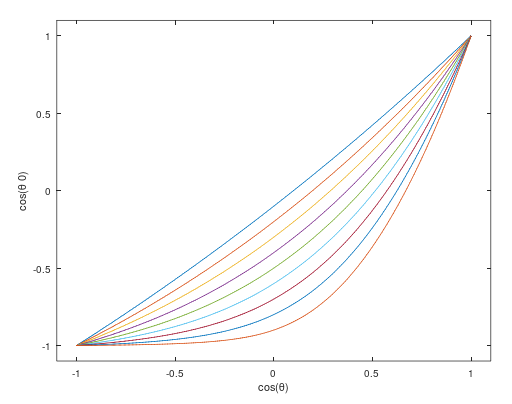
\includegraphics[width=10cm]{chapter_04_paragraph_16_fig_14a}
		\caption{\'Equation (\ref{EQ:16_6}) dans le cas $v_{0} > V$ pour $\dfrac{V}{v_{0}}$ compris entre 0.1 et 0.9 avec un pas de 0.1 et pour $0 < \theta < \pi$}\label{FIG:4_14A}
	\end{center}
\end{figure}

Dans le cas o\`u $v_{0} > V$, le vecteur $\vec{v}$ ne croise le cercle de rayon $v_{0}$ qu'en un unique point et comme il est n\'ecessaire de choisir $\theta_{0} = 0$ quand $\theta = 0$, la solution (\ref{EQ:16_6}) se r\'eduit \`a $\cos\theta_{0} = -\dfrac{V}{v_{0}}\sin^{2}\theta + \cos\theta\sqrt{1 - \dfrac{V^{2}}{v_{0}^{2}}\sin^{2}\theta}$. Ce cas est repr\'esent\'e sur la figure (\ref{FIG:4_14A}) Dans le cas o\`u $v_{0} < V$, le vecteur $\vec{v}$ croise le m\^eme cercle en deux points, B et C sur la figure correspondante (\ref{FIG:4_14}) tel qu'il existe alors deux valeurs de $\theta_{0}$ pour chaque valeur de $\theta$. Ce cas est illustr\'e sur la figure (\ref{FIG:4_14B}).

\begin{figure}[htb!]
	\begin{center}
		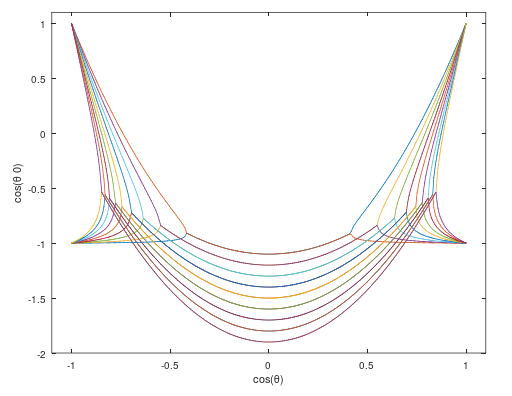
\includegraphics[width=10cm]{chapter_04_paragraph_16_fig_14b}
		\caption{Deux solutions de l\'equation (\ref{EQ:16_6}) dans le cas $v_{0} < V$ pour $\dfrac{V}{v_{0}}$ compris entre 1.1 et 1.9 avec un pas de 0.1 et pour $0 < \theta < \pi$}\label{FIG:4_14B}
	\end{center}
\end{figure}

Dans la plupart des applications physiques, ce sont de nombreuses particules qui se d\'esint\`egrent et il faut alors raisonner en termes de distribution, en \'energie, en impulsion, en directions, etc. Prenons d\'esormais l'hypoth\`ese de particules initiales orient\'ees de mani\`ere chaotique, i.e. en moyenne de fa\c{c}on isotrope. Dans le r\'ef\'erentiel <<~c~>>, l'isotropie est conserv\'ee apr\`es les d\'esint\'egrations et les particules r\'esultantes de m\^eme esp\`ece ont alors la m\^eme \'energie et la r\'epartition des trajectoires est isotrope. L'orientation chaotique peut se traduire comme la quantit\'e de particules traversant un angle solide\footnote{Par d\'efinition, un \'el\'ement d'angle solide est d\'efini par $\mathrm{d}^{2}\Omega = \dfrac{\vec{r}\cdot\vec{n}}{r^{3}}\mathrm{d}^{2}S$ avec $\vec{r}$ le vecteur rayon et $\vec{n}$ le vecteur normale de l'\'el\'ement de surface $\mathrm{d}^{2}S$. Dans le cadre d'une sph\`ere, nous avons $\mathrm{d}^{2}S = r\mathrm{d}\theta r\sin\theta\mathrm{d}\varphi$ et par cons\'equent $\mathrm{d}^{2}\Omega = \sin\theta\mathrm{d}\theta\mathrm{d}\varphi$ ou encore $\mathrm{d}\Omega = 2\pi\sin\theta\mathrm{d}\theta$.} $\mathrm{d}\omega_{0}$ qui est proportionnelle \`a la grandeur de cet \'el\'ement soit $\frac{\mathrm{d}\omega_{0}}{4\pi}$. Dans le cadre d'une sph\`ere, $\mathrm{d}\omega_{0} = 2\pi\sin\theta_{0}\mathrm{d}\theta_{0}$, donc :
\be
	\dfrac{\mathrm{d}\omega_{0}}{4\pi} = \dfrac{1}{2}\pi\sin\theta_{0}\mathrm{d}\theta_{0} \label{EQ:16_7}
\ee